%\documentclass{article}
%\usepackage{graphicx,subfigure}
%\begin{document}

\begin{figure}[!h]
  \centering
   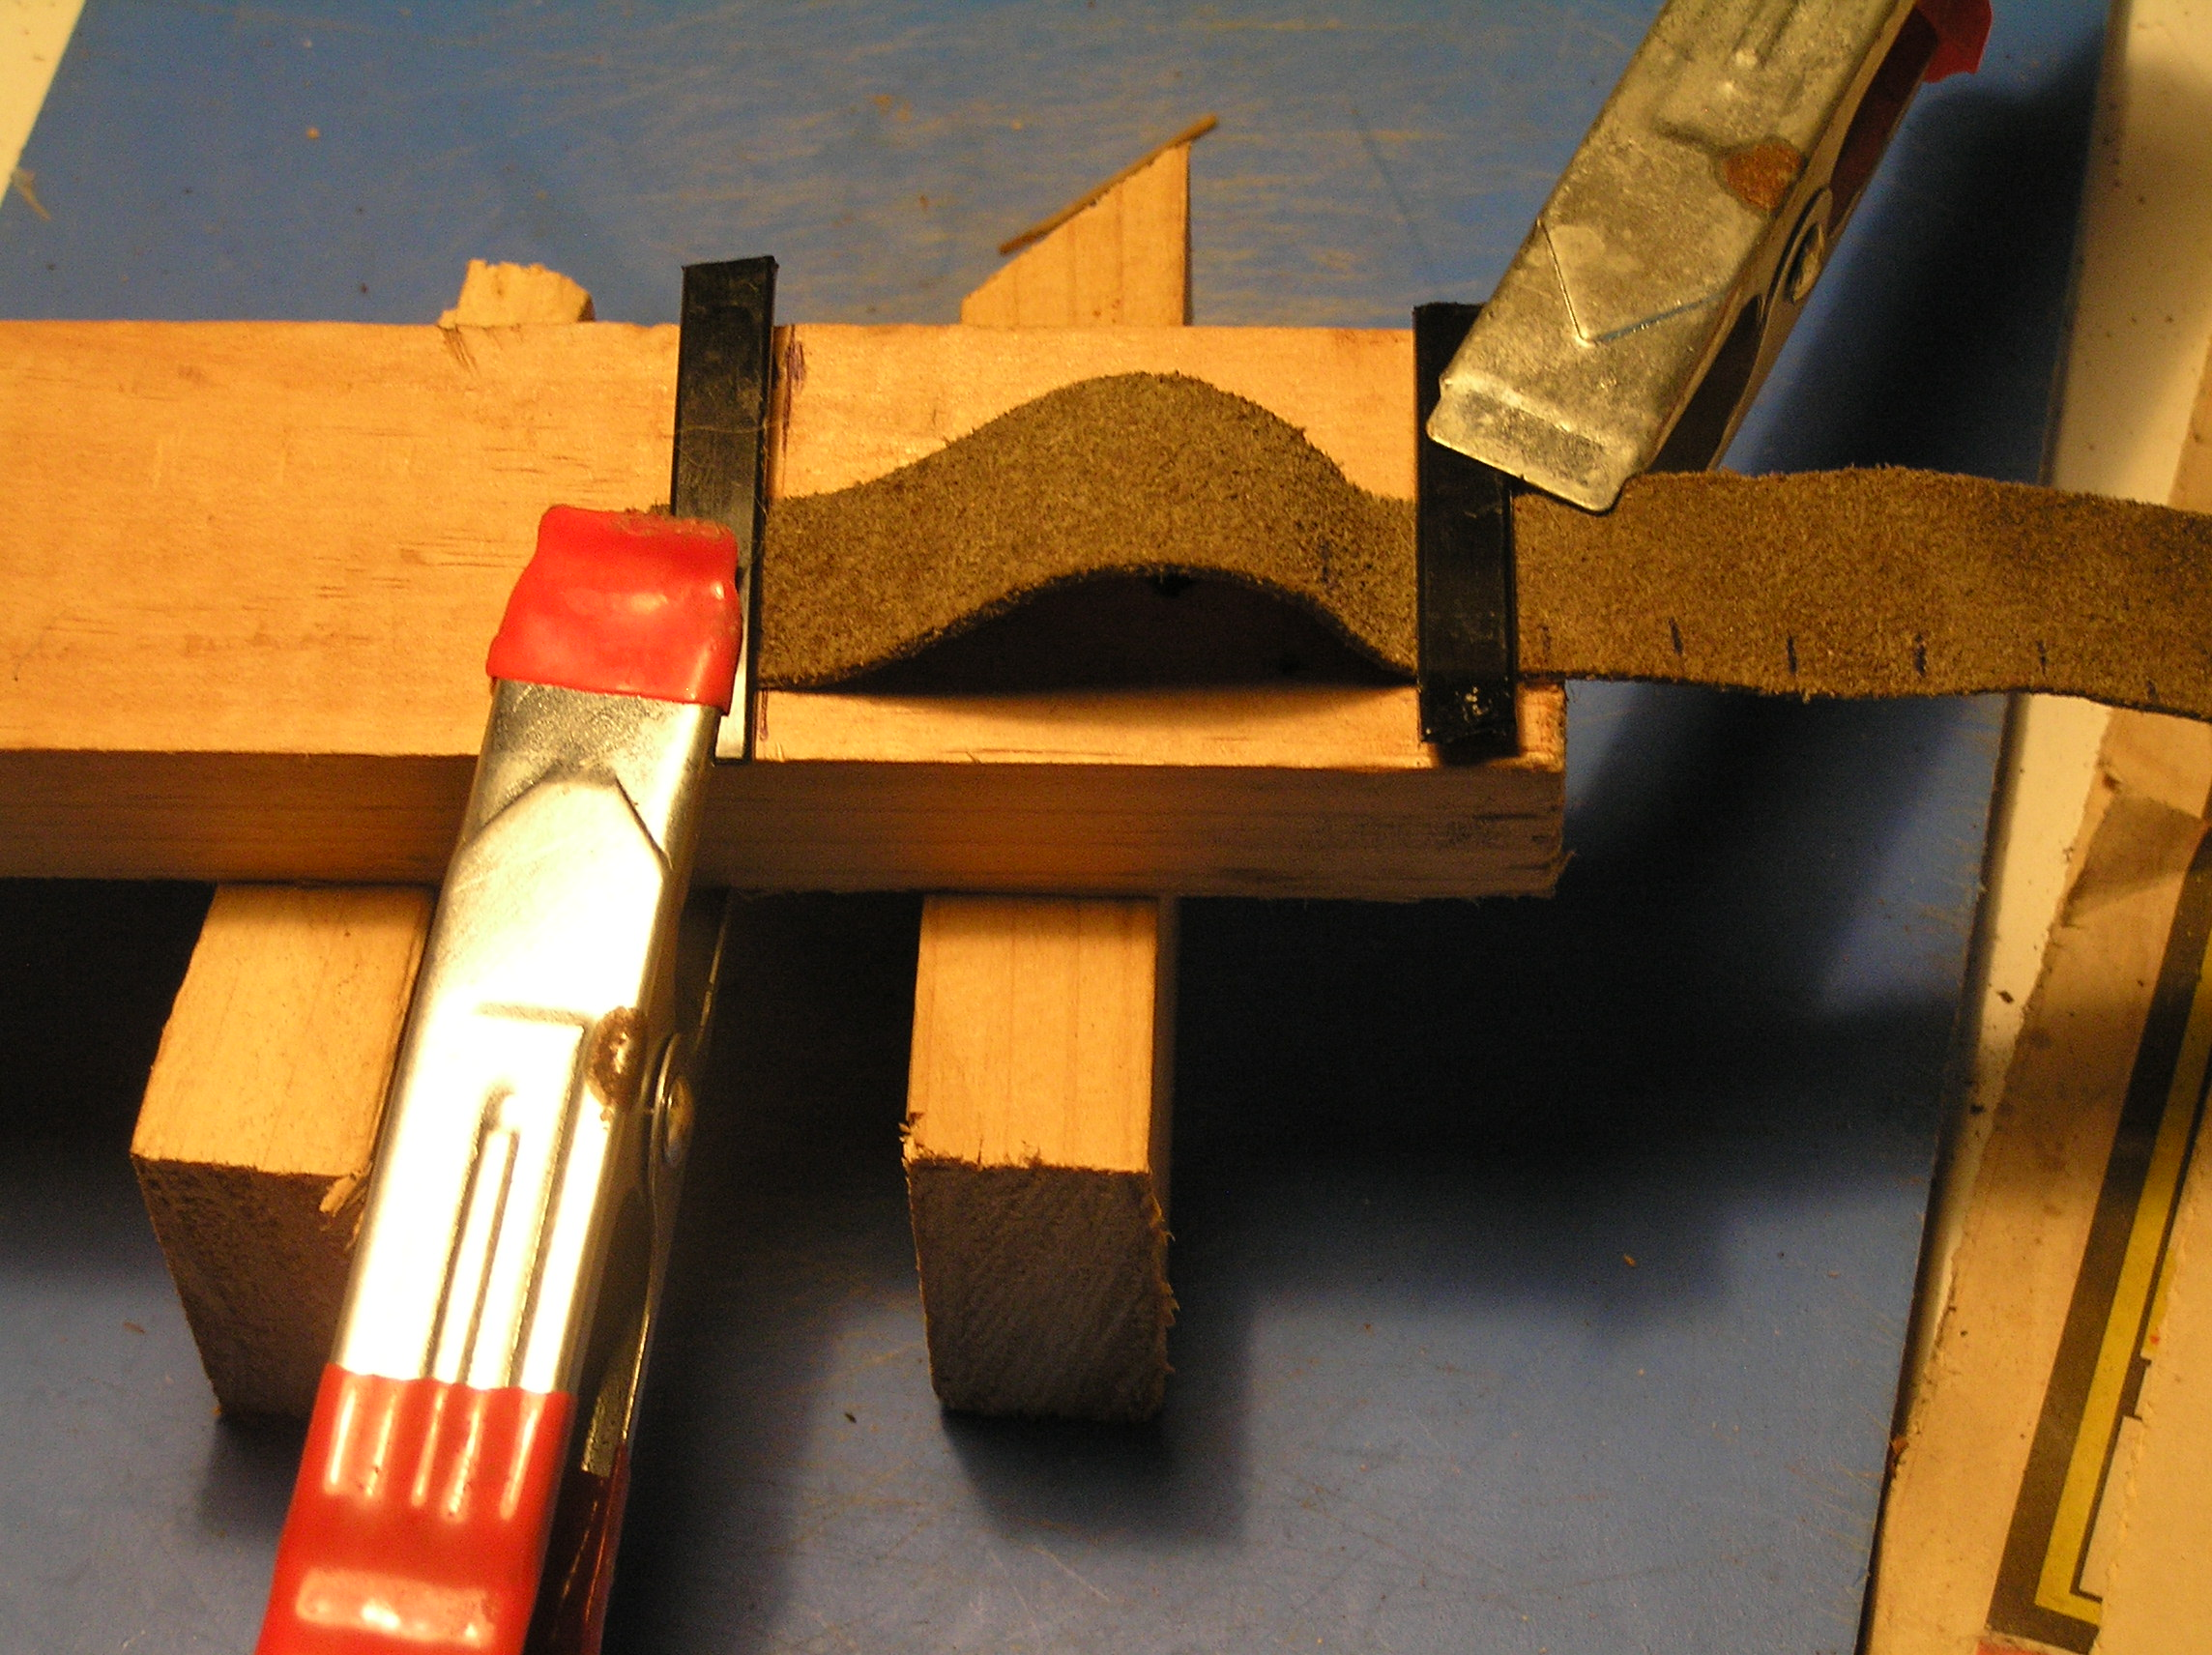
\includegraphics[width=0.9\textwidth]{images/P1010004.JPG}
  \caption{Physical model with a 50mm strip of leather clamped at 0mm and 60mm to a board at positions 0mm and 50mm. The leather represents dermis. The board represents subdermal tissue. This demonstrates fold formation when the leather strip has 10mm of expansion (over the original 50mm), a 20 percent expansion.}
  \label{fig:model2}
\end{figure}

%\end{document}

